\documentclass[a4paper]{article}

\usepackage[utf8]{inputenc}

% ***********************************************************
% ******************* PHYSICS HEADER ************************
% ***********************************************************
% Version 2
%\documentclass[11pt]{article} 
\usepackage{amsmath} % AMS Math Package
\usepackage{amsthm} % Theorem Formatting
\usepackage{amssymb}	% Math symbols such as \mathbb
\usepackage{graphicx} % Allows for eps images
\usepackage{multicol} % Allows for multiple columns
\usepackage[dvips,letterpaper,margin=0.75in,bottom=0.5in]{geometry}
 % Sets margins and page size
\pagestyle{empty} % Removes page numbers
\makeatletter % Need for anything that contains an @ command 
\renewcommand{\maketitle} % Redefine maketitle to conserve space
{ \begingroup \vskip 10pt \begin{center} \large {\bf \@title}
	\vskip 10pt \large \@author \hskip 20pt \@date \end{center}
  \vskip 10pt \endgroup \setcounter{footnote}{0} }
\makeatother % End of region containing @ commands
\renewcommand{\labelenumi}{(\alph{enumi})} % Use letters for enumerate
% \DeclareMathOperator{\Sample}{Sample}
\let\vaccent=\v % rename builtin command \v{} to \vaccent{}
\renewcommand{\v}[1]{\ensuremath{\mathbf{#1}}} % for vectors
\newcommand{\gv}[1]{\ensuremath{\mbox{\boldmath$ #1 $}}} 
% for vectors of Greek letters
\newcommand{\uv}[1]{\ensuremath{\mathbf{\hat{#1}}}} % for unit vector
\newcommand{\abs}[1]{\left| #1 \right|} % for absolute value
\newcommand{\avg}[1]{\left< #1 \right>} % for average
\let\underdot=\d % rename builtin command \d{} to \underdot{}
\renewcommand{\d}[2]{\frac{d #1}{d #2}} % for derivatives
\newcommand{\dd}[2]{\frac{d^2 #1}{d #2^2}} % for double derivatives
\newcommand{\pd}[2]{\frac{\partial #1}{\partial #2}} 
% for partial derivatives
\newcommand{\pdd}[2]{\frac{\partial^2 #1}{\partial #2^2}} 
% for double partial derivatives
\newcommand{\pdc}[3]{\left( \frac{\partial #1}{\partial #2}
 \right)_{#3}} % for thermodynamic partial derivatives
\newcommand{\ket}[1]{\left| #1 \right>} % for Dirac bras
\newcommand{\bra}[1]{\left< #1 \right|} % for Dirac kets
\newcommand{\braket}[2]{\left< #1 \vphantom{#2} \right|
 \left. #2 \vphantom{#1} \right>} % for Dirac brackets
\newcommand{\matrixel}[3]{\left< #1 \vphantom{#2#3} \right|
 #2 \left| #3 \vphantom{#1#2} \right>} % for Dirac matrix elements
\newcommand{\grad}[1]{\gv{\nabla} #1} % for gradient
\let\divsymb=\div % rename builtin command \div to \divsymb
\renewcommand{\div}[1]{\gv{\nabla} \cdot #1} % for divergence
\newcommand{\curl}[1]{\gv{\nabla} \times #1} % for curl
\let\baraccent=\= % rename builtin command \= to \baraccent
\renewcommand{\=}[1]{\stackrel{#1}{=}} % for putting numbers above =
\newtheorem{prop}{Proposition}
\newtheorem{thm}{Theorem}[section]
\newtheorem{lem}[thm]{Lemma}
\theoremstyle{definition}
\newtheorem{dfn}{Definition}
\theoremstyle{remark}
\newtheorem*{rmk}{Remark}

% ***********************************************************
% ********************** END HEADER *************************
% ***********************************************************

\usepackage{braket}

\usepackage[swedish]{babel}

\usepackage{rotating}

\usepackage{multirow}

% \usepackage{graphicx}

\title{\textbf{FYSA31:} Two Electron System}

\author{Author: Jonas Wess\'en}

\date{October 14th, 2011}

\begin{document}

\maketitle

\thispagestyle{empty}

\newpage

\section{Introduction}

\section{Theory}

\subsection{LS-coupling and the Land\'e Interval Rule}

In the following section, the $LS$-coupling will be described. An description of its required approximations is presented, and finally the Land\'e Interval Rule is described which in the experiment will be used for investigation of whether $LS$-coupling is valid or not.

The phenomena of \textit{fine structure} in an atom arises from the coupling of the intrinsic angular momentum of the electron (carried by its spin) and its orbital angular momentum, which gives a contribution $H_{LS}$ to the total Hamiltonian $H_{tot}$ of the system. Due to its spin, an electron has a magnetic dipole moment $\vec{\mu_s}$ that takes the form

\begin{equation}

\vec{\mu_s} = -g_s \frac{\mu_b}{\hbar} \vec{s}

\end{equation}

where $g_s \approx 2$ is the gyromagnetic ratio, $\mu_b = e \hbar / 2m_e$ the Bohr magnetron and $\vec{s}$ the spin angular momentum with $|\vec{s}|=\sqrt{s(s+1)} \hbar$ and $\hat{z} \cdot \vec{s} = \hbar m_s$ where $s=1/2$ and $m_s = \pm 1/2$ since the electron is a fermion. If several electrons are involved, the total spin angular momentum $\vec{S}$ will be the vector sum of the individual spin angular momenta, causing the magnetic dipole moment

\begin{equation}

\vec{\mu_S} = -g_s \frac{\mu_b}{\hbar} \vec{S}. \label{muS}

\end{equation}

$\vec{S}$ is described by the quantum number $S$ in the same sense that $\vec{s}$ is described by $s$. There are only two allowed directions for the electron spin ("up" or "down"), meaning that $\vec{S}$ is nothing but the sum of up's and down's. Suppose there are $n$ valence electrons bound to the atom (the other electrons form closed shells with no resulting orbital or spin angular momentum). The minimum value $S$ can take is when the spin of as many electrons as possible cancel (all electrons if $n$ is even, and all except one if $n$ is odd). The maximum $S$ occurs when all the spins align. This can be summarized in

\begin{equation}

S = \frac{1-(-1)^{n+1}}{2} , \dots , \frac{n}{2}.

\end{equation}

where the dots indicate integer steps (flipping a spin from $-1/2$ to $+1/2$ results in an integer change of the total spin). For the two electron system ($n=2$) with electron spins $s_1$ and $s_2$, this description is equivalent to the more familiar

\begin{equation}

S = |s_1 - s_2|, \dots, |s_1 + s_2|

\end{equation}

giving $S=0$ or $S=1$.

An single orbiting charge (with charge $dq$) will classically produce a magnetic field $d\vec{B}$ proportional to the angular momentum $\vec{l}$ of the charge. This can be realized by considering Biot-Savat's law for a moving charge

\begin{equation}

d\vec{B} = \frac{\mu_0}{4\pi} \cdot \frac{dq}{dt} \cdot \frac{d\vec{x} \times \vec{r}}{r^3} \label{BS}

\end{equation}

where $d\vec{x}$ is the infinitesimal length element in the direction of the motion and $\vec{r}$ the position vector of the charge. After some simple algebraic manipulation, eq. (\ref{BS}) is rearranged to

\begin{equation}

d\vec{B} = \frac{\mu_0 dq}{4\pi mr^3} \cdot \vec{l} \propto \vec{l} \label{propL}

\end{equation}

where it has been used that $\vec{l}=m \cdot d\vec{x}/dt \times \vec{r}$ where $m$ is the mass of the charge\footnote{The magnitude of the magnetic field $\vec{B}$ due to an orbiting electron in an atom can be estimated by, in eq. (\ref{propL}), letting $d\vec{B}\rightarrow \vec{B}$, $m\rightarrow m_e$, $dq \rightarrow e$, $r \rightarrow r_B$ (Bohr radius) and $|\vec{l}|\rightarrow \hbar$ (of course $|\vec{l}|=\hbar \sqrt{l(l+1)}$ where $l$ is the orbital quantum number, but this is just an estimate of the order of magnitude for the $\vec{B}$-field). This gives $B \approx 12.5$T which is much stronger than most "macroscopic" magnetic fields in our every day life. However, it is quite easily shown that the coulomb attraction between two elementary charges at Bohr radius is about $10^7$ times greater than the magnetic force ($\vec{F}=q\vec{v}\times \vec{B}$) of an electron in an atom put in this field, which justifies the assumption that electron-electron interaction due to their magnetic fields is normally not relevant for $LS$ coupling.}.

By considering an atom from the electrons point of view, the nucleus will orbit the electron, thus creating a magnetic field proportional to the nucleus angular momentum (which only differs by a factor $m_N/m_e$, where $m_N$ is the mass of the nucleus, from the angular momentum of the electron in the nucleus frame of reference). From classical physics, it can be shown that a dipole moment $\vec{\mu}$ in a magnetic field $\vec{B}$ tries to align itself with the field, giving a potential energy described by $E=-\vec{\mu}\cdot\vec{B}$. In the electrons frame of reference, different energy levels will therefor arise, depending on the angle between the magnetic moment and the magnetic field, and these energy levels must of course still be there when switching back to the more natural frame of reference with the nucleus at the origin. Since the $\vec{B}$-field in the frame of reference of the electron, is proportional to $\vec{l}$ (and therefor also the potential energy contribution $-\vec{\mu}\cdot\vec{B}$), the energy levels we observe (in the nucleus frame of reference) must also have energies proportional to $\vec{l}$.

Since $\vec{\mu_s}$ is proportional to $\vec{s}$, the energy contribution for spin-orbit interaction, for an atom with one electron, must be proportional to the product $\vec{l} \cdot \vec{s}$. When spin-orbit coupling in an atom with more than one electron, it is assumed that the energy contribution is proportional to $\vec{L}\cdot\vec{S}$, where $\vec{L}$ is the total orbital angular momentum, described by the quantum number $L$ which is constructed from the $l$'s of the electrons, in the same manner as $S$ is constructed from the $s$'s. The quantum mechanical representation of this is a term $H_{LS}$ in the Hamiltonian of the system, i.e.

\begin{equation}

H_{tot} = H_0 + H_{LS} = H_0 + C \vec{L}\cdot\vec{S}

\end{equation}

where $H_0$ is the Hamilton operator which includes all other energy contributions other than the $LS$-contribution. Here, it is assumed that $-\vec{\mu}\cdot\vec{B}\propto\vec{L}\vec{S}$, which is a good approximation in most cases (see [2] for a more detailed discussion).

To deal with the strange operator $\vec{L}\cdot\vec{S}$, the operator $\vec{J}$, defined as

\begin{equation}

\vec{J} \equiv \vec{L} + \vec{S},

\end{equation}

is used to rewrite $\vec{L}\cdot\vec{S}$ to

\begin{equation}

\vec{L}\vec{S}=\frac{1}{2}(\vec{J}^2-\vec{L}^2-\vec{S}^2)

\end{equation}

Since $\vec{J}$, $\vec{L}$ and $\vec{S}$ all are angular momentum operators\footnote{There is no doubt that $\vec{L}$ and $\vec{S}$ are angular momentum operators, but it is not completely obvious that $\vec{J}$ is, given its definition. An angular momentum operator is any operator $\vec{A}=(A_x,A_y,A_z)$ which satisfies the commutator relation $[A_i,A_j]= \epsilon_{ijk} i \hbar A_k$ where $\epsilon_{ijk}=1$ if $ijk$ is a cyclic permutation of $xyz$, $\epsilon_{ijk}=-1$ if $ijk$ is an anti-cyclic permutation and $\epsilon_{ijk}=0$ otherwise. Since $\vec{J} =(J_x,J_y,J_z)=\vec{L} + \vec{S} = (L_x+S_x,L_y+S_y,L_z+S_z)$, and $\vec{L}$ and $\vec{S}$ are angular momentum operators, it holds that $[J_i,J_j]=[L_i+S_i,L_j+S_j]=[L_i,L_k] + [S_i,S_j] + [L_i,S_j] + [S_i,L_j] = \epsilon_{ijk} i \hbar L_k + \epsilon_{ijk} i \hbar S_k + 0 + 0 = \epsilon_{ijk} i \hbar J_k$, i.e. $\vec{J}$ must be an angular momentum operator. Note that the proof required $[L_i,S_j]=0$ for all $i$ and $j$, which might not have been true if $\vec{L}$ and $\vec{S}$ were some other angular momentum operators, i.e. the sum of two angular momentum operators is not necessarily another angular momentum operator.} that commute with each other, there exists a complete set of eigenstates $\Ket{J,L,S}$ such that

\begin{eqnarray}

\vec{J}^2 \Ket{J,L,S} = J(J+1) \hbar^2 \Ket{J,L,S}, \label{J} \\

\vec{L}^2 \Ket{J,L,S} = L(L+1) \hbar^2 \Ket{J,L,S}, \\

\vec{S}^2 \Ket{J,L,S} = S(S+1) \hbar^2 \Ket{J,L,S}. \label{S}

\end{eqnarray}

Treating the spin-orbit interaction as a perturbation, the energy contribution to an eigenstate $\Ket{J,L,S}$ to first order is

\begin{equation}

E_{LS}^{(1)} = \Bra{J,L,S} C \vec{L}\cdot\vec{S} \Ket{J,L,S} = \frac{C}{2} \Bra{J,L,S} (\vec{J}^2-\vec{L}^2-\vec{S}^2) \Ket{J,L,S}.

\end{equation}

Plugging in eq.(\ref{J})-(\ref{S}), one gets

\begin{equation}

E_{LS}^{(1)}(J,L,S) = \frac{C}{2} (J(J+1) - L(L+1) - S(S+1)).

\end{equation}

One may now consider the energy difference $\Delta E$ between the two levels $\Ket{J,L,S}$ and $\Ket{J-1,L,S}$:

\begin{equation}

\Delta E = \frac{C}{2} ( J(J+1) - (J-1)J ) = C J,

\end{equation}

i.e. the energy splitting between two adjacent levels is proportional to the $J$-value of the upper level. This is known as the \textit{Land\'e's interval rule}, and can be a useful test for have how good the $LS$-approximation is. By measuring the energy splitting between different levels with same $L$ and $S$, and divide by $J$, one can investigate how good the $LS$-approximation is for the specific levels.

\subsection{Forbidden transitions}

In the conducted experiments, it will be shown that transitions happen which actually are forbidden by the LS approximation. An attempt to explain these transitions will hereby follow.

Since the energy contribution from spin-orbit interaction is treated as a first order perturbation in the LS approximation, one might expect that the obtained "LS states" (let's call them $\ket{LS_n}$) only are approximately equal to the actual eigenstates to the full Hamiltonian (hereby denoted $\ket{\Psi_n}$). Still the set $\{ \ket{LS_n} \}$ still form a complete basis since they are formed from a set of commutating operators, meaning that \textit{any} state, including any $\ket{\Psi_n}$, can be expressed as a linear combination of $\ket{LS_n}$-states. For a particular $\ket{\Psi_n}$ it thereby holds that

\begin{equation}

\ket{\Psi_n} = \sum_m a_{nm} \ket{LS_m}.

\end{equation}

For most states, where the LS coupling is valid, the coefficients $a_{nm} = \delta_{nm}$ (where $\delta_{mn}$ is the Kronecker delta). Though, for a state $\ket{\Psi_\alpha}$ that happens to have a bad LS coupling, one might have

\begin{equation}

\ket{\Psi_\alpha} = a \ket{LS_\alpha} + b \ket{LS_\beta}

\end{equation}

for two LS states $\ket{LS_\alpha}$ and $\ket{LS_\beta}$, with $b$ small, but not negligible. Consider another state $\ket{LS_\gamma} = \ket{\Psi_\gamma}$ for which that the transition

\begin{equation}

\ket{LS_\gamma} \to \ket{LS_\beta}

\end{equation}

is valid by the LS approximation, but that the transition $\ket{LS_\gamma} \to \ket{LS_\alpha}$ is forbidden\footnote{For example, $\ket{LS_\alpha}$ might be a singlet, while $\ket{LS_\beta}$ and $\ket{LS_\gamma}$ are triplets.}. The transition probability between $\ket{\Psi_\alpha}$ and $\ket{\Psi_\gamma}$ will then be

\begin{equation}

P_{\alpha \to \gamma} \propto |\bra{\Psi_\gamma}-e\vec{r}\ket{\Psi_\alpha}|^2 = |a\bra{LS_\gamma}-e\vec{r}\ket{LS_\alpha} + b\bra{LS_\gamma}-e\vec{r}\ket{LS_\beta}|^2 = |b|^2 |\bra{LS_\gamma}-e\vec{r}\ket{LS_\beta}|^2 \neq 0.

\end{equation}

\subsection{The Hollow Cathode and the Fourier Transform Spectrometer}

\begin{figure}[htb!]

\label{HC}

\begin{center}

\scalebox{.5}{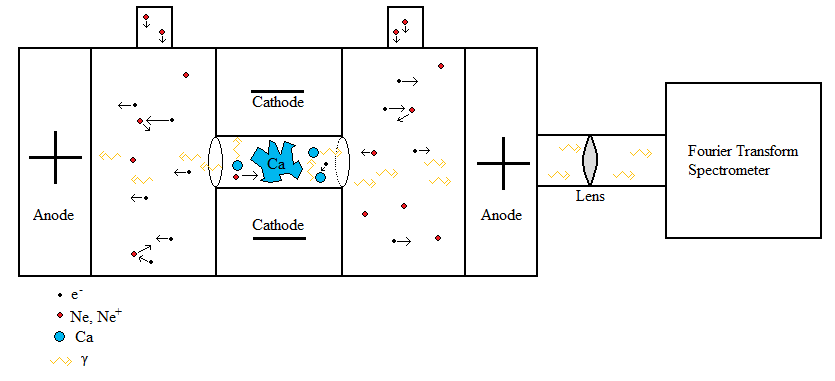
\includegraphics{HollowCathode}}

\end{center}

\caption{\textit{Simplified picture of the hollow cathode.}}

\end{figure}

Figure 1 shows the tube-shaped hollow cathode, which in this experiment is used to produce the light spectra of Ca I. A sample of Ca I is put inside a tube surrounded by a cathode. In the surroundings, a carrier gas (in this case Ne), is present. When a voltage is put over the tube, electrons will drive towards the anodes at the ends of the tube. Some of these electrons will collide with the Ne atoms and ionize them, provided that the electron had enough energy. The ionized Ne$^+$ will then accelerate towards the cathode in the middle, some of them towards the middle of the cathode where the Ca I sample is placed. The heavy Ne$^+$ atoms will then collide with the Ca sample, causing Ca atoms to leave the sample (this process is called sputtering). The free Ca atoms will thereby, mostly via collisions with electrons, start to radiate (equally in all directions). Some of the radiation will be collected in a lens, before entering the Fourier Transform Spectrometer (shown in figure 2).

\begin{figure}[htb!]

\label{FTS}

\begin{center}

\scalebox{.5}{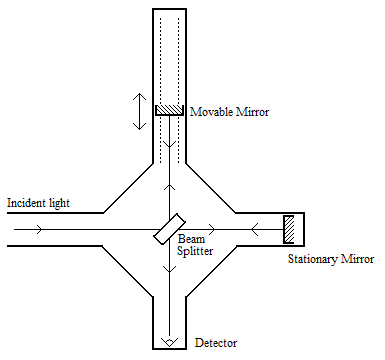
\includegraphics{FTS}}

\end{center}

\caption{\textit{The Fourier Transform Spectrometer.}}

\end{figure}

The Fourier Transform Spectrometer is very similar to the commonly used Michelson interferometer. The incident light is divided into two parts by going through a 45$^\circ$ beam splitter. Each beam is reflected back through the beam splitter, and registered in a detector as shown in figure 2. Depending on the difference between the optical path distances $\Delta l$ for the two beams, they will interfere differently (constructive interference when $\Delta l = m \lambda$ where $m$ is an integer and $\lambda$ the wavelength, and destructive interference when $\Delta l = (m+ 1/2) \lambda$). One of the mirrors can be moved back and forth, making it possible to investigate the interference pattern at different wavelengths. Let $x$ indicate the path distance. By detecting the intensity $I$ as a function of $x$, the different wavenumbers $\sigma$ of spectra is obtained by taking the Fourier transform of $I$:

\begin{equation}

\hat{I}(\sigma ) = \frac{1}{\sqrt{2\pi }} \int_{-\infty}^{\infty} e^{-i\sigma x} I(x) dx,

\end{equation}

giving a peak at each wavenumber of the spectra. Due to Doppler shift of the light, the peaks in the spectra will be approximately Gaussian, i.e. a narrow continuum of light with different wavelengths. Consider the registered intensity around one particular wavenumber $\sigma_i$. When $x=0$, light with any wavenumber will interfere constructively. However, when $x\approx 1/ \sigma_i$, only light with wavenumber close to $\sigma_i$ interfere constructively, which will manifest itself as an intensity decrease (compared to $x=0$). After another period, i.e. $x=2/\sigma_i$, more of the light will cancel, thus giving a lower intensity. When the mirror is moved far enough, the registered intensity will be constant with respect to $x$, meaning that the signal does not contain any information about $\sigma_i$ at all \footnote{One could of course try to show this by calculating the inverse Fourier transform of $\hat{I}(\sigma)$, where $\hat{I}$ is a Gaussian peak in the wavenumber, but this tuns out to be rather messy, and not very instructive for the purpose of this report.} The signal $I(x)$ will therefor be a damped cosine function with wavenumber $\sigma_i$. It turns out ([REFERENS?]) that it is not profitable to move the mirror further than

\begin{equation}

L = \frac{1.2}{2\cdot \delta \sigma} %I'm not sure about this formula! I just vagely remember it from the Spectrophysics book which I don't own.

\end{equation}

where $\delta \sigma$ is the broadening of the line (in terms of wavenumbers).

\begin{figure}[htb!]

\label{cos}

\begin{center}

\scalebox{.4}{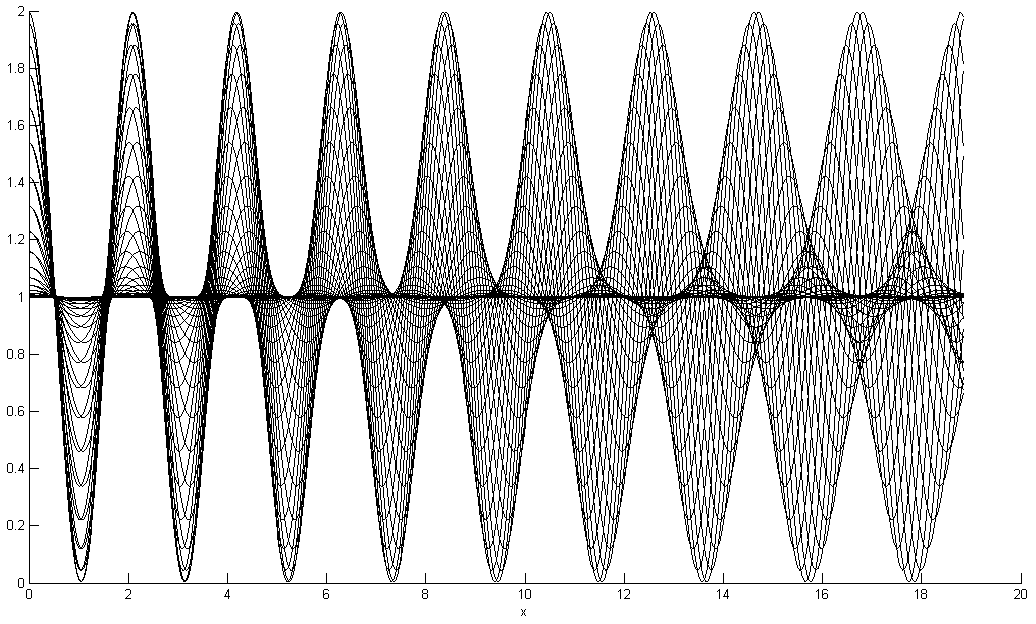
\includegraphics{cos}}

\end{center}

\caption{\textit{Due to line broadening, the Fourier Transform Spectrometer will register a Gaussian-distributed continuum of light with different wave numbers. The figure simultaneously shows several (of course not a continuum!) cosine functions with Gaussian-distributed amplitudes, corresponding to some of the light frequencies that are registered by the Fourier Transform Spectrometer. The figure uses arbitrary units for $x$ and $I$.}}

\end{figure}

\begin{figure}[htb!]

\label{sumCos}

\begin{center}

\scalebox{.4}{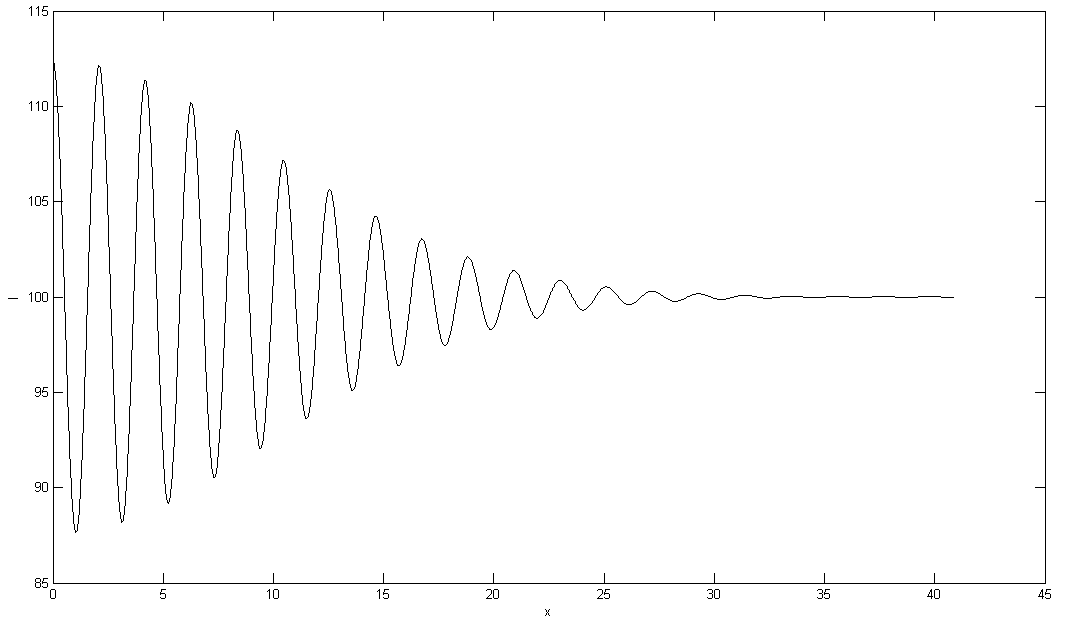
\includegraphics{sumCos}}

\end{center}

\caption{\textit{A sum of cosine functions (in this case the functions depicted in figure 3) with different wavenumbers and Gaussian-distributed amplitudes (intensities) will approximately be a damped cosine function with wave number corresponding to the strongest intensity. This is signal the Fourier Transform Spectrometer records, meaning that after a certain value of $x$ (optical path difference of the two light beams), the signal does not contain any information. The figure uses arbitrary units for $x$ and $I$.}}

\end{figure}

%It holds that

%\begin{equation}

%I(x) = \frac{1}{\sqrt{2\pi }} \int_{-\infty}^{\infty} e^{-i\sigma x} \hat{I}(\sigma ) d \sigma.

%\end{equation}

%In the spectra, $\hat{I}(\sigma )$ will be a narrow Gaussian distribution around each wavenumber $\sigma_i$ with variance $D^2$, i.e.

%\begin{equation}

%\hat{I}(\sigma ) =

%\end{equation}

%When $x=0$, constructive interference will occur at all wavelengths. The actual spectrum will of course consist of %(approximately Gaussian) peaks at different wavenumbers $\sigma$, but lets first consider

\section{Experiment \& Results}

In the ground state, $^{20}_{40}Ca$ has the configuration

$[\mathrm{Ar}]4s^2$. In the 1st excited state, one of the 4s electrons is

excited to the 3d state, giving rise to the LS terms $^1D_2$ and

$^3D_{1,2,3}$.

In another excited state, the atom has the configuration 3d4p, and

hence the following LS terms:

\[

\begin{array}{c}

^1P_1, ^3P_{0, 1, 2}\\

^1D_2, ^3D_{1,2,3} \\

^1F_3, ^3F_{2,3,4}

\end{array}

\]

During this experiment, the transitions $3d4p\,^3D_{1,2,3} \to

3d4s\,^3D_{1,2,3}$ and $3d4p\,^3F_{2,3,4} \to 3d4s\,^3D_{1,2,3}$ are

studied.

\subsection{Transitions $3d4p\,^3D_{1,2,3} \to 3d4s\,^3D_{1,2,3}$}

The anticipated $3d4p\,^3D_{1,2,3} \to 3d4s\,^3D_{1,2,3}$ transitions

are illustrated in figure \ref{fig:transition1}.

\begin{figure}[htb!]

\centering

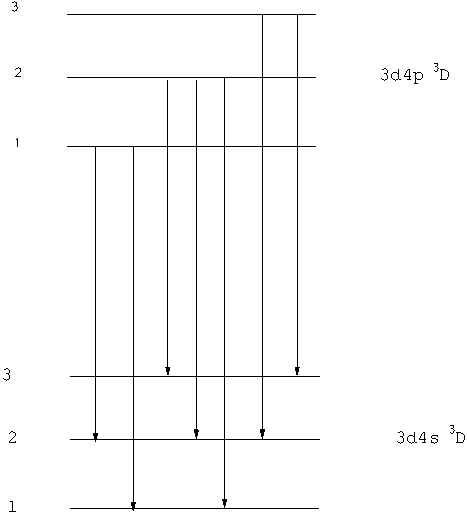
\includegraphics[scale=0.35]{transition1}

\caption{The $3d4p\,^3D_{1,2,3} \to 3d4s\,^3D_{1,2,3}$ transitions}

\label{fig:transition1}

\end{figure}

These transitions have been worked out by following the selection

rules that govern which transitions are possible:

\begin{itemize}

\item $\Delta L = 0, \pm 1$, but $0 \to 0$ is forbidden;

\item $\Delta J = 0, \pm 1$, but $0 \to 0$ is forbidden;

\item $\Delta S = 0$

\item for individual electrons, $\Delta l = \pm 1$, i.e. the parity

must change.

\end{itemize}

Under the guidance of the supervisor, the region of the spectrum with

wave number from 17840 $\rm cm^{-1}$ to 17950 $\rm cm^{-1}$ is

searched to find the peaks corresponding to the 7 transitions. The

results are shown in tables \ref{tab:transitions11} and \ref{tab:transitions12}.

\begin{table}[htb!]

\centering

\begin{tabular}{c|c|c|c}

\hline

No. & position ($\rm cm^{-1}$) & Intensity & Width ($\rm cm^{-1}$) \\

\hline

1 & 17843.115 & 0.030 & 0.053 \\

2 & 17848.004 & 0.031 & 0.053 \\

3 & 17857.011 & 0.081 & 0.053 \\

4 & 17869.839 & 0.117 & 0.054 \\

5 & 17883.738 & 0.029 & 0.053 \\

6 & 17888.097 & 0.189 & 0.054 \\

7 & 17909.833 & 0.029 & 0.053 \\

\hline

\end{tabular}

\caption{Peaks of the $3d4p\,^3D_{1,2,3} \to 3d4s\,^3D_{1,2,3}$

transitions for experiment 1.}

\label{tab:transitions11}

\end{table}

\begin{table}[htb!]

\centering

\begin{tabular}{c|c|c|c}

\hline

No. & position ($\rm cm^{-1}$) & Intensity & Width ($\rm cm^{-1}$) \\

\hline

1 & 17843.112 & 0.019 & 0.052 \\

2 & 17848.001 & 0.020 & 0.052 \\

3 & 17857.009 & 0.054 & 0.053 \\

4 & 17869.837 & 0.079 & 0.053 \\

5 & 17883.735 & 0.019 & 0.053 \\

6 & 17888.094 & 0.131 & 0.053 \\

7 & 17909.831 & 0.019 & 0.053 \\

\hline

\end{tabular}

\caption{Peaks of the $3d4p\,^3D_{1,2,3} \to 3d4s\,^3D_{1,2,3}$

transitions for experiment 2.}

\label{tab:transitions12}

\end{table}

In order to associate the measured peaks with the theoretically

predicted transitions, one has to calculate the theoretical transition

energies and compare them with the experimental results. The

easiest is, however, to calculate and compare the {\it relative}

intensities of the transitions. For that purpose, the intensity of the

transition $3d4p\;^3\mathrm{D}_3 \to 3d4s\;^3\mathrm{D}_3$ is assigned

the value 100, while the intensity of the other lines are represented

as a percentage of it. The calculation is carried out using the

formula\footnote{This formula might be derived by adding the time-dependent perturbation $h=-e \vec{r} \cdot \hat{e} E_0 \cos{\omega t}$ to the Hamiltonian (corresponding to the oscillating electric field with frequency $\omega$ and amplitude $E_0$ in direction $\hat{e}$ of a photon), whereby applying some time-dependent perturbation theory.}

\[

S_{if} \propto |\matrixel{\psi_i}{e\vec{r}}{\psi_f}|^2

\]

And the result is listed in table \ref{tab:intensity1}

\begin{table}[htb!]

\centering

\begin{tabular}{cc|c|c|c|}

\cline{3-5}

& & \multicolumn{3}{c|}{$3d4p ^3D$}\\

\cline{3-5}

& & 3 & 2 & 1\\

\hline

\multicolumn{1}{|c|}{\multirow{3}{*}{$3d4s ^3D$}} & 3 & 100 & 12.5 & \\

\multicolumn{1}{|c|}{} & 2 & 12.5 & 55.8 & 12.05 \\

\multicolumn{1}{|c|}{} & 1 & & 12.05 & 36.16 \\

\hline

\end{tabular}

\caption{Theoretically predicted relative intensities of the

$3d4p\,^3D_{1,2,3} \to 3d4s\,^3D_{1,2,3}$ transitions}

\label{tab:intensity1}

\end{table}

Comparing table \ref{tab:intensity1} with tables \ref{tab:transitions11} and \ref{tab:transitions12},

it is immediately clear that line No.6 corresponds to transition $3

\to 3$, since it has the highest intensity and the $3 \to 3$

transition is predicted to have the highest intensity.

Similarly, one can establish that line No.4 corresponds to $2 \to 2$,

since it has the second highest intensity, and that line No.3

corresponds to $1 \to 1$, since it has the third highest intensity.

The other 4 lines have similar intensities and cannot be discerned in

the same way. The lab manual gives the wave number of the involved

levels:

\begin{itemize}

\item $3d4s\,^3D_1$: 20 335.360 cm$^{-1}$

\item $3d4s\,^3D_2$: 20 349.260 cm$^{-1}$

\item $3d4s\,^3D_3$: 20 371.000 cm$^{-1}$

\end{itemize}

Combining these data with the position of the identified lines No.6,

No.4 and No.3, one can work out the wave number of the other levels as

well as the position of the other lines. Eventually, the correspondence

between the lines and the transitions are established. The calculated wave

numbers of the $3d4p ^3D$ terms for the two experiments are shown below, and the

transition-line correspondence is shown below:

Experiment 1:

\begin{itemize}

\item $3d4p\,^3D_1$: 38192.371 cm$^{-1}$

\item $3d4p\,^3D_2$: 38219.099 cm$^{-1}$

\item $3d4p\,^3D_3$: 38259.097 cm$^{-1}$

\end{itemize}

Experiment 2:

\begin{itemize}

\item $3d4p\,^3D_1$: 38192.369 cm$^{-1}$

\item $3d4p\,^3D_2$: 38219.097 cm$^{-1}$

\item $3d4p\,^3D_3$: 38259.094 cm$^{-1}$

\end{itemize}

\begin{table}

\centering

\begin{tabular}{c|c}

No. & Transition ($J_1 \to J_2$)\\

\hline

1 & $1 \to 2$ \\

2 & $2 \to 3$ \\

3 & $1 \to 1$ \\

4 & $2 \to 2$\\

5 & $2 \to 1$\\

6 & $3 \to 3$\\

7 & $3 \to 2$\\

\hline

\end{tabular}

\caption{Line-transition correspondence}

\label{tab:line-transition1}

\end{table}

Now the relative intensities of the lines can be calculated from the

experimental data (table \ref{tab:exp-intensity11} and \ref{tab:exp-intensity12}):

\begin{table}[htb!]

\centering

\begin{tabular}{cc|c|c|c|}

\cline{3-5}

& & \multicolumn{3}{c|}{$3d4p ^3D$}\\

\cline{3-5}

& & 3 & 2 & 1\\

\hline

\multicolumn{1}{|c|}{\multirow{3}{*}{$3d4s ^3D$}} & 3 & 100 (100) &

15.27 (12.5) & \\

\multicolumn{1}{|c|}{} & 2 & 14.50 (12.5) & 60.31 (55.8) & 14.50 (12.05) \\

\multicolumn{1}{|c|}{} & 1 & & 16.36 (12.05) & 41.22 (36.16) \\

\hline

\end{tabular}

\caption{\it Experimentally determined relative intensities, in experiment 1, of the

$3d4p\,^3D_{1,2,3} \to 3d4s\,^3D_{1,2,3}$ transitions. The

theoretical counterparts are surrounded by a parenthesis.}

\label{tab:exp-intensity11}

\end{table}

\begin{table}[htb!]

\centering

\begin{tabular}{cc|c|c|c|}

\cline{3-5}

& & \multicolumn{3}{c|}{$3d4p ^3D$}\\

\cline{3-5}

& & 3 & 2 & 1\\

\hline

\multicolumn{1}{|c|}{\multirow{3}{*}{$3d4s ^3D$}} & 3 & 100 (100) &

16.40 (12.5) & \\

\multicolumn{1}{|c|}{} & 2 & 15.34 (12.5) & 61.90 (55.8) & 15.87 (12.05) \\

\multicolumn{1}{|c|}{} & 1 & & 15.34 (12.05) & 42.86 (36.16) \\

\hline

\end{tabular}

\caption{\it Experimentally determined relative intensities, in experiment 2, of the

$3d4p\,^3D_{1,2,3} \to 3d4s\,^3D_{1,2,3}$ transitions. The

theoretical counterparts are surrounded by a parenthesis.}

\label{tab:exp-intensity12}

\end{table}

Land\'e's interval rule states that, if LS-coupling is valid, the

energy splitting between two LS terms can be calculated as

\[

\Delta E = C J_u

\]

where C is a constant and $J_u$ is the J value of the upper level.

In order to verify or repudiate this statement, the following is

calculated for experiment 1:

\begin{eqnarray*}

\frac{\Delta E_{3,2}}{3} &=& \frac{E(3d4p\,^3D_3) -

E(3d4p\,^3D_2)}{3}\\

&=& \frac{38259.097 - 38219.099}{3} \\

&=& 13.33 \\

\frac{\Delta E_{2,1}}{2} &=& \frac{E(3d4p\,^3D_2) -

E(3d4p\,^3D_1)}{3}\\

&=& \frac{38219.099 - 38192.371}{2} \\

&=& 13.36

\end{eqnarray*}

In the same manner, the following is calculated for experiment 2:

\begin{eqnarray*}

\frac{\Delta E_{3,2}}{3} &=& 13.33, \\

\frac{\Delta E_{2,1}}{2} &=& 13.36.

\end{eqnarray*}

$\frac{\Delta E_{3,2}}{3}$ and $\frac{\Delta E_{2,1}}{2}$ are rather

close, thus the validity of Land\'e's interval rule is affirmed.

Another interesting thing observed in tables \ref{tab:exp-intensity11} and \ref{tab:exp-intensity12}

is that the experimental intensities are generally greater than their

theoretical counterparts. A review of the theoretical treatment

suggests this is an effect of self absorption that has not been

considered so far: Photons emitted during the de-excitation process

have to pass by other atoms in the sample and hence are subject to

scattering and absorption. The cross section of the absorption is

apparently larger for the more intense photons. Therefore, the higher

the intensity, the greater the loss of intensity by self

absorption. As the most intense line is used as a reference of

intensity, the other lines all appear more intense.

\subsection{Transitions $3d4p\,^3F_{2,3,4} \to 3d4s\,^3D_{1,2,3}$}

The anticipated $3d4p\,^3F_{2,3,4} \to 3d4s\,^3D_{1,2,3}$ transitions

are illustrated in figure \ref{fig:transition2}.

\begin{figure}[htb!]

\centering

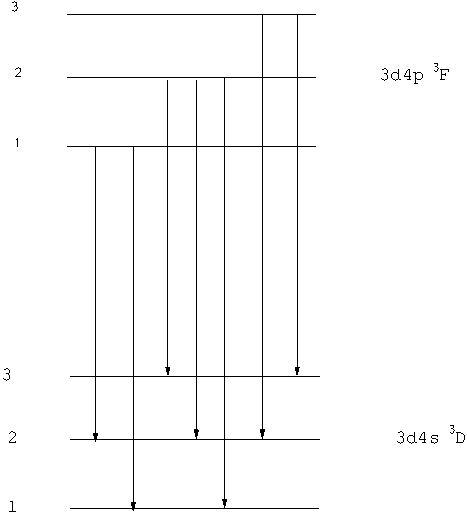
\includegraphics[scale=0.35]{transition2}

\caption{The $3d4p\,^3F_{2,3,4} \to 3d4s\,^3D_{1,2,3}$ transitions}

\label{fig:transition2}

\end{figure}

As with the $3d4p\,^3D_{1,2,3} \to 3d4s\,^3D_{1,2,3}$ transitions, the supervisor

helps locate the right region to search for the corresponding peaks. In total, 10 peaks are

found (table \ref{tab:transitions21}) in experiment 1, and 8 peaks in experiment 2 (table \ref{tab:transitions22}):

\begin{table}[htb!]

\centering

\begin{tabular}{c|c|c|c}

\hline

No. & position ($\rm cm^{-1}$) & Intensity & Width ($\rm cm^{-1}$) \\

\hline

1 & 15359.440 & 0.001 & 0.048 \\

2 & 15381.178 & 0.044 & 0.046 \\

3 & 15395.077 & 0.197 & 0.047 \\

4 & 15447.695 & 0.055 & 0.046 \\

5 & 15464.383 & 0.000790 & 0.046 \\

6 & 15469.431 & 0.355 & 0.047 \\

7 & 15486.126 & 0.013 & 0.045 \\

8 & 15500.029 & 0.082 & 0.047 \\

9 & 15512.288 & 0.013 & 0.064 \\

10 & 15525.872 & 0.456 & 0.048 \\

\hline

\end{tabular}

\caption{Peaks of the $3d4p\,^3F_{2,3,4} \to 3d4s\,^3D_{1,2,3}$ transitions for experiment 1.}

\label{tab:transitions21}

\end{table}

\begin{table}[htb!]

\centering

\begin{tabular}{c|c|c|c}

\hline

No. & position ($\rm cm^{-1}$) & Intensity & Width ($\rm cm^{-1}$) \\

\hline

1 & 15381.177 & 0.029 & 0.046 \\

2 & 15395.077 & 0.130 & 0.046 \\

3 & 15447.697 & 0.035 & 0.046 \\

4 & 15469.431 & 0.241 & 0.046 \\

5 & 15486.125 & 0.008 & 0.045 \\

6 & 15500.025 & 0.055 & 0.046 \\

7 & 15512.286 & 0.013 & 0.062 \\

8 & 15525.873 & 0.311 & 0.047 \\

\hline

\end{tabular}

\caption{Peaks of the $3d4p\,^3F_{2,3,4} \to 3d4s\,^3D_{1,2,3}$ transitions for experiment 2.}

\label{tab:transitions22}

\end{table}

As has been done for the last group of transitions, the first task is to associate

the transitions with the measured peaks. Theoretical calculations give the following

for the relative intensity of the peaks: (table \ref{tab:intensity2})

\begin{table}[htb!]

\centering

\begin{tabular}{cc|c|c|c|}

\cline{3-5}

& & \multicolumn{3}{c|}{$3d4p ^3F$}\\

\cline{3-5}

& & 4 & 3 & 2\\

\hline

\multicolumn{1}{|c|}{\multirow{3}{*}{$3d4s ^3D$}} & 3 & 100 & 8.64 & 0.25\\

\multicolumn{1}{|c|}{} & 2 & & 69.19 & 8.64 \\

\multicolumn{1}{|c|}{} & 1 & & & 46.67 \\

\hline

\end{tabular}

\caption{\it Theoretically predicted relative intensities of the

$3d4p\,^3F_{4,3,2} \to 3d4s\,^3D_{1,2,3}$ transitions.}

\label{tab:intensity2}

\end{table}

The strongest three lines are immediately identifiable by their

intensities in experiment 1:

\begin{itemize}

\item $4 \to 3$: No. 10

\item $3 \to 2$: No. 6

\item $2 \to 1$: No. 3

\end{itemize}

and in experiment 2:

\begin{itemize}

\item $4 \to 3$: No. 8

\item $3 \to 2$: No. 4

\item $2 \to 1$: No. 2

\end{itemize}

Then, as before, one can calculate the wave numbers of the

$3d4p\,^3F_{4,3,2}$ terms using the wave numbers of the

$3d4s\,^3D_{1,2,3}$ terms given in the lab manual. The results are

as follows:

Experiment 1:

\begin{itemize}

\item $3d4p\,^3F_{4}$: 35896.872 $\rm cm^{-1}$

\item $3d4p\,^3F_{3}$: 35818.691 $\rm cm^{-1}$

\item $3d4p\,^3F_{2}$: 35730.437 $\rm cm^{-1}$

\end{itemize}

Experiment 2:

\begin{itemize}

\item $3d4p\,^3F_{4}$: 35896.873 $\rm cm^{-1}$

\item $3d4p\,^3F_{3}$: 35818.691 $\rm cm^{-1}$

\item $3d4p\,^3F_{2}$: 35730.537 $\rm cm^{-1}$

\end{itemize}

Then some of the transitions can be associated with the peaks, as shown in tables \ref{tab:line-transition21} and \ref{tab:line-transition22}.

\begin{table}[htb!]

\centering

\begin{tabular}{c|c}

\hline

No. & Transition ($J_1 \to J_2$)\\

\hline

1 & $2 \to 3$ \\

2 & $2 \to 2$ \\

3 & $2 \to 1$ \\

4 & $3 \to 3$ \\

6 & $3 \to 2$ \\

10 & $4 \to 3$\\

\hline

\end{tabular}

\caption{Line-transition correspondence in experiment 1.}

\label{tab:line-transition21}

\end{table}

In experiment 2, the line corresponding to the transition $2 \to 3$ is not detected due to its low intensity.

\begin{table}[htb!]

\centering

\begin{tabular}{c|c}

\hline

No. & Transition ($J_1 \to J_2$)\\

\hline

1 & $2 \to 2$ \\

2 & $2 \to 1$ \\

3 & $3 \to 3$ \\

4 & $3 \to 2$ \\

8 & $4 \to 3$ \\

\hline

\end{tabular}

\caption{Line-transition correspondence in experiment 2.}

\label{tab:line-transition22}

\end{table}

\begin{table}[htb!]

\centering

\begin{tabular}{cc|c|c|c|}

\cline{3-5}

& & \multicolumn{3}{c|}{$3d4p ^3F$}\\

\cline{3-5}

& & 4 & 3 & 2\\

\hline

\multicolumn{1}{|c|}{\multirow{3}{*}{$3d4s ^3D$}} & 3 & 100 (100) &

12.06 (8.64) & 0.21 (0.25) \\

\multicolumn{1}{|c|}{} & 2 & & 77.85 (69.19) & 9.65 (8.64)\\

\multicolumn{1}{|c|}{} & 1 & & & 43.20 (46.67) \\

\hline

\end{tabular}

\caption{\it Experimentally determined relative intensities, in experiment 1, of the

$3d4p\,^3F_{4,3,2} \to 3d4s\,^3D_{1,2,3}$ transitions. The

theoretical counterparts are surrounded by a parenthesis.}

\label{tab:exp-intensity21}

\end{table}

A careful inspection reveals that the difference in wave number between line No. 5 and No.7 is very close to that between level $3d4s ^{2}D$ and $3d4s ^{3}D$, and the difference between line No. 7 and No.8 is also very close to that between level $3d4s ^{1}D$ and $3d4s ^{2}D$. So there is a good reason to believe that an extra level exists, and transitions from this level to the $3d4s$ levels have happened. Adding the wave numbers of transitions No.5 , No.7 and No.8 to those of the $3d4s$ levels gives, consistently, the wave number of the unexpected level: 35835,386 cm$^{-1}$.

Another thing to notice is that Land\'e's interval rule no longer holds true when it comes to the splitting between the $3d4p$ levels:

\begin{eqnarray*}

A_{4,3} &=& \frac{35896.872 - 35818.691}{4} \\

&=& 19.5 \\

A_{3,2} &=& \frac{35818.691 - 35730.437}{3} \\

&=& 29.4 \\

\end{eqnarray*}

The existance of an unexpected level and the violation of Land\'e's interval rule clearly suggest that LS coupling is no longer a good approximation, and prompt the the use of second-order perturbation theory:

\[

E''_{so} = \frac{|\langle \psi_1 | H_{so} | \psi_2 \rangle|^2}{E_1 - E_2}

\]

With this method, one finds the ``raised'' $3d4p\;^1D_2$ state to be the previously unexpected level. This concludes the experiment.

\begin{table}[htb!]

\centering

\begin{tabular}{cc|c|c|c|}

\cline{3-5}

& & \multicolumn{3}{c|}{$3d4p ^3F$}\\

\cline{3-5}

& & 4 & 3 & 2\\

\hline

\multicolumn{1}{|c|}{\multirow{3}{*}{$3d4s ^3D$}} & 3 & 100 (100) &

11.18 (8.64) & 0.00 (0.25) \\

\multicolumn{1}{|c|}{} & 2 & & 77.00 (69.19) & 9.27 (8.64)\\

\multicolumn{1}{|c|}{} & 1 & & & 41.53 (46.67) \\

\hline

\end{tabular}

\caption{\it Experimentally determined relative intensities, in experiment 2, of the

$3d4p\,^3F_{4,3,2} \to 3d4s\,^3D_{1,2,3}$ transitions. The

theoretical counterparts are surrounded by a parenthesis.}

\label{tab:exp-intensity22}

\end{table}

\section{Source Reference}

\begin{enumerate}

\item \textit{Two Electron Systems} (Lab Manual)

\item \textit{Modern Quantum Mechanics}, J.J. Sakurai, Jim Napolitano.

\end{enumerate}

\end{document}